\documentclass[12pt]{article}
\pagestyle{empty}
\usepackage{amsmath, amssymb, amsthm}
\usepackage{latexsym, epsfig, ulem, cancel, multicol, hyperref}
\usepackage{graphicx, tikz, subfigure,pgfplots}
\usepackage[margin=1in]{geometry}
\setlength{\parindent}{0pt}
\usepackage{multirow}
\usepackage{mathtools}


\newcommand{\R}{\mathbb{R}}
\newcommand{\dydx}{\frac{dy}{dx}}
\usepackage{verbatim}
\usepackage{tikz}
\usepackage{pgfplots}

\newcommand{\wsnumber}{1}
\newcommand{\wstopic}{Vectors}
\pgfplotsset{
    every linear axis/.append style={
       axis x line=center,
       axis y line=center,
       xlabel={$x$},
       ylabel={$y$}
    },
    every axis plot/.append style={thick,mark=none}
}
\tikzset{
    point/.style={circle,draw,fill,minimum width=0.3ex,inner sep=0pt,outer sep=0pt},
    every label/.append style={black}
}


\usepackage[margin=1in]{geometry}
\usepackage{amsmath, amssymb, amsthm, graphicx, hyperref}
\usepackage{enumerate}
\usepackage{fancyhdr}
\usepackage{multirow, multicol}
\usepackage{tikz}
\pagestyle{fancy}
\fancyhead[RO]{Dennis Li}
\fancyhead[LO]{MA-UY 3113 Complex Variables and Linear Algebra }
\usepackage{comment}
\newif\ifshow
\showfalse

\ifshow
  \newenvironment{solution}{\textbf{Solution.}}{}
\else
  \excludecomment{solution}
\fi

\renewcommand{\thefootnote}{\fnsymbol{footnote}}
\usepackage{comment}


\newtheorem*{remark}{Remark}


\begin{document}

\begin{center}
\ifshow
  \textbf{\Large Homework 2 Solution}\\
\else
  \textbf{\Large Homework 2}\\
\fi
Due: Friday February 16, by 11:59pm,\\via Gradescope\\
\end{center}

\hrule

\vspace{0.2cm}

\begin{enumerate}[$\bullet$]
\item  {\textbf{\textit{Note that you must assign a page to each problem you submit.}}}   Gradescope has great YouTube videos available on how to submit homework.  \textit{\textbf{Failure to submit homework correctly will result in a zero on homework.}}
\item Problems that appear with the notation \colorbox{yellow}{$\ast$} will require you to TeX your solution.  If no highlighted star appears, then a hand written solution is OK.  
\item Late homework is not accepted.  Lateness due to technical issues will not be excused.  
\end{enumerate}

\hrule

\vspace{0.5cm}



\begin{enumerate}


\item(8 points) Find $Arg(z)$ for
\begin{enumerate}
    \item  \colorbox{yellow}{$\ast$}   $z = \frac{3 + 4i}{-2+i}$
    \[
    z=\frac{(3+4i)(-2-i)}{5}
    \]
    \[
    z=\frac{-2-11i}{5}
    \]
    since $z_1 = -2-11i$ is along the same line as $z_2=-\frac{1}{5}(2+11i)$\\ in the complex plain\\
    we may argue that $Arg(z_1)=Arg(z_2)$\\
    \[
    Arg(z_1)=arctan(\frac{11}{2})-\pi
    \]
    Thus $Arg(z_2) = arctan(\frac{11}{2})-\pi$
    
    \item   $z = \frac{-3 + 4i}{-2+i}$\\
    let $z_3=\frac{-3 + 4i}{-2+i}$, \[
    z_3=\frac{(-3+4i)(-2-i)}{5}
    \]
    \[
    z_3=\frac{10-5i}{5}=2-i
    \]
    Thus the argument is\[
    Arg(z_3)=arctan(-\frac{1}{2})
    \]
    since arctan is an odd function, we can also write it as \[
    Arg(z_3)=-arctan(\frac{1}{2})
    \]
    \item   $z = \frac{-3 - 4i}{-2+i}$\\
    let $z_4 = \frac{-3 - 4i}{-2+i}$\\
    we can see that $-z_2=z_4$, which is effectively rotating it $\pi$ rad.\\
    Thus we may argue that\[
    Arg(z_4)=Arg(z_2)+\pi= arctan(\frac{11}{2})
    \]
    \item   $z = \frac{3 - 4i}{-2+i}$\\
    Similarly, we let $z_5=\frac{3 - 4i}{-2+i}$ and notice that $-z_3=z_5$\\
    Thus we may make the same argument as previous that\[
    Arg(z_5)=Arg(z_3)+\pi=-arctan(\frac{1}{2})+\pi
    \]
\end{enumerate}


\begin{remark}
    Recall that $Arg(z)$ is the principle argument of $z$.  
\end{remark}

\item (5 points)  \colorbox{yellow}{$\ast$}  Find all solutions to the equation 
\[  
w^{12} = -2 - 5i
\]
\textbf{Solution:}\\
let $z_1=-2-5i$, The modulus of $z_1$ is\[
|z_1| = \sqrt{4+25}=\sqrt{29}
\]
and the argument of $z_1$ is\[
arg(z_1)=arctan(\frac{5}{2})-\pi
\]
we can write $z_1$ in its polar form as\[
z_1=\sqrt{29}\exp{(i[arctan(\frac{5}{2})-\pi])}
\]
now let $w=Re^{i\theta}$, and\[
w^{12}=R^{12}\exp{(12i\theta)}=\sqrt{29}\exp{(i[arctan(\frac{5}{2})-\pi])}
\]
we have\[
R=29^{\frac{1}{24}}
\]
and\[
12\theta + 2\pi k=arctan(\frac{5}{2})-\pi
\]
\[
\theta=\frac{1}{12}(arctan(\frac{5}{2})-\pi-2\pi k), k\in\mathbb{Z}
\]
Thus, the solution can be written as\[
w=29^{\frac{1}{24}}\exp{(\frac{1}{12}i(arctan(\frac{5}{2})-\pi-2\pi k))},  k\in\{0,1,2...,11\}
\]

\begin{remark}
    There are exactly 12 solutions.  
\end{remark}

\item (5 points)  Find the 11 roots of unity.  That is, find all solutions to the equation $w^{11} = 1$.  
\textbf{Solution:}\\
The 11 roots of unity of $w^{11}=1$ can be described as 11 evenly distributed on the unit circle on the complex plain\\
let\[
w=R\exp{(i\theta)}
\]
where $R=1$, and $\theta=\frac{2\pi k}{11}, k\in\mathbb{Z}$
Thus the roots can be written as\[
w=\exp{(i\frac{2\pi k}{11})}, k\in\{0,1,2...,11\}
\]
\begin{remark}
    There are exactly 11 solutions.  
\end{remark}

\item (4 points)  Sketch the regions in the complex plane associated to the inequalities 
\begin{enumerate}
    \item All $z$ such that $|z - 1 + 2i| \geq 1$.\\
    \textbf{Solution:}\\
    let $z=x+iy$, we have\[
    |(x-1)+i(y+2)|\geq1
    \]
    by definition of the modulus, we have
    \[
    \sqrt{(x-1)^2+(y+2)^2}\geq1
    \]
    squaring both side
    \[
    (x-1)^2+(y+2)^2 \geq 1
    \]
    the domain can be expressed as\[
    \{(x,y)\in\mathbb{R}^2|(x-1)^2+(y+2)^2 \geq 1\}
    \]
    we can thus determine region such that this inequality stands to be (see next page)\\
    
\begin{figure}
    \centering
    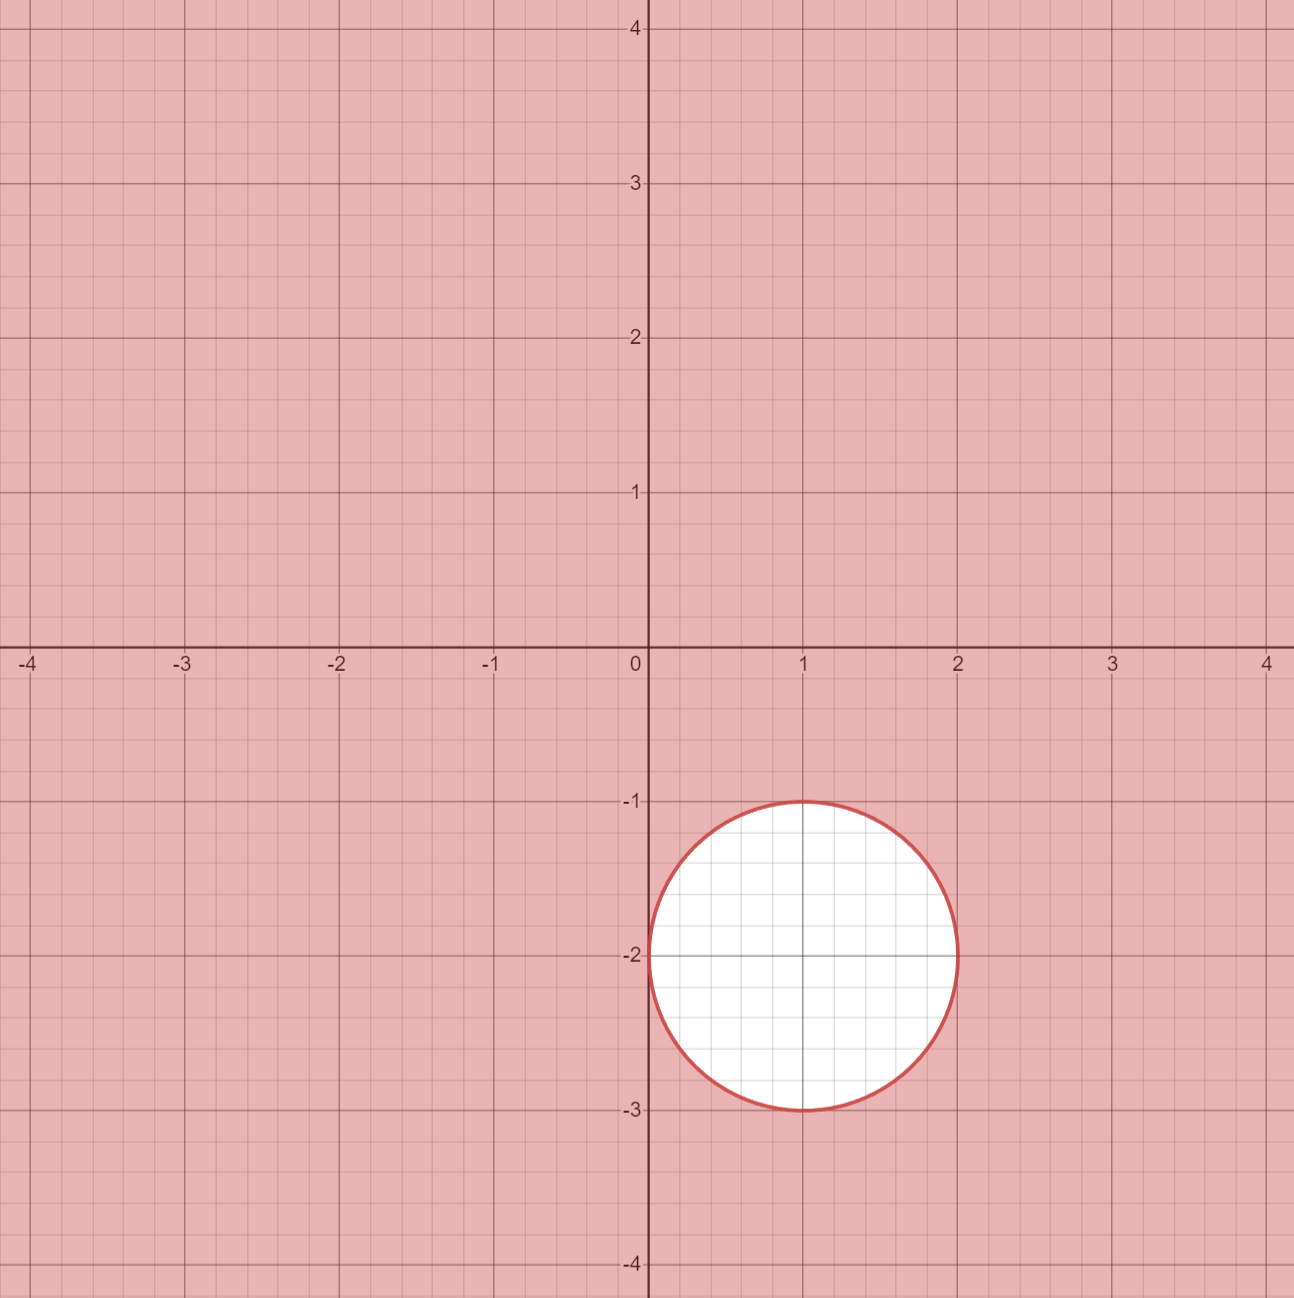
\includegraphics[width=0.5\linewidth]{pictures/4a_pic.png}
    \caption{Region in Question 4(a)}
    \label{fig:4(a)}
\end{figure}
\\  
    \item All $z$ such that $Re(z) < 3Im(z) $.\\
    \textbf{Solution:}\\
    let $z=x+iy$, such that $Re(z)=x$ and $Im(z)=y$\\
    we have the domain\[
    \{(x,y)\in\mathbb{R}^2|x<3y\}
    \]
    Thus we can plot this inequality as below (see next page)
    \begin{figure}
        \centering
        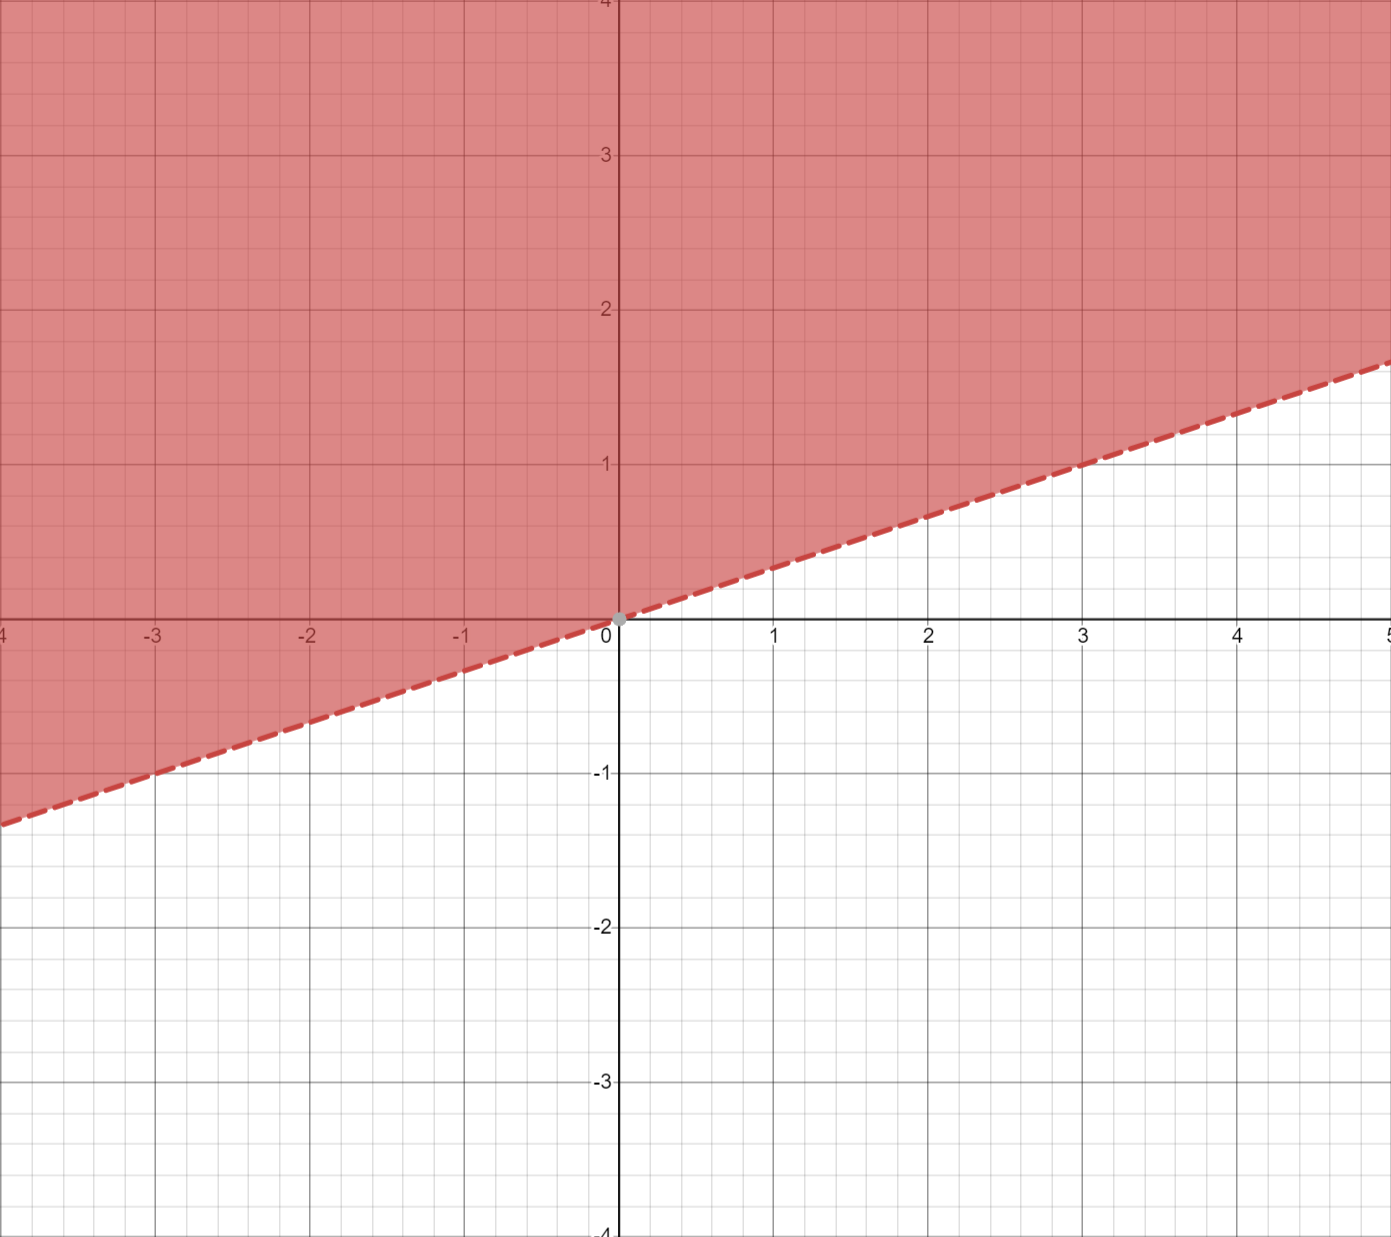
\includegraphics[width=0.5\linewidth]{pictures/4b_pic.png}
        \caption{Region in Question 4(b)}
        \label{fig:4(b)}
    \end{figure}

    
\end{enumerate}

\item (6 points) Describe the domains (no sketch needed) for the functions 
\begin{enumerate}
    \item $f(z) = \frac{z}{z - \bar{z} } $.\\
    \textbf{Solution:}\\
    This complex function exists if\\
    \[
    z-\Bar{z}\neq 0
    \]
    let $z=x+iy$ and $\Bar{z}=x-iy$, we can obtain\[
    x+iy-(x-iy)\neq 0
    \]
    \[
    2iy\neq 0
    \]
    so the domain of $f(z)$ or $f(x,y)$ is
    \[
    \{(x,y)\in\mathbb{R}^2|y\neq0\}
    \]
    

    
    \item $f(z) = \frac{1}{z^{11} - 1}$.\\
    \textbf{Solutions:}\\
    For $f(z)$ to exist, $z^{11}-1\neq0$\\
    we can see that
    \[
    \nexists f(z) \iff z^{11}-1=0
    \]
    evaluate:\[
    z^{11}=1
    \]
    we can see this is the 11th roots of unity. Thus, we can determine:\[
    z=e^{i\frac{2\pi k}{11}},k\in\{0,1,2...10\}
    \]
    Thus we can determine that the domain of $f(z)$ is\[
    \
    \{z\in\mathbb{C},k\in \mathbb{Z}|z\neq e^{i\frac{2\pi k}{11}},0\leq k\leq 10\}
    \]
\end{enumerate}


\item (6 points)  Find $Re(f)$ and $Im(f)$ for the functions 
\begin{enumerate}
    \item  \colorbox{yellow}{$\ast$}  $f(z) = \frac{z}{z+1}$.\\
    \textbf{Solution:}\\
    let $z=x+iy$, the function can be written as\[
    f(x,y)=\frac{x+iy}{(x+1)+iy}
    \]
    multiplying the denominator by its complex conjugate, we have\[
    f(x,y)=\frac{(x+iy)(x+1-iy)}{(x+1)^2+y^2}
    \]
    simplifying this expression, we can obtain\[
    f(x,y)=\frac{x^2+x+y^2}{x^2+2x+y^2+1}+\frac{iy}{x^2+2x+y^2+1}
    \]
    Thus\[
    Re(f)=\frac{x^2+x+y^2}{x^2+2x+y^2+1}
    \]
    \[
    Im(f)=\frac{y}{x^2+2x+y^2+1}
    \]
    
    \item $f(z) = z^{3} + 2z -5$.  \\
    \textbf{Solution:}\\
    let $z=x+iy$, the function can be written as\[
    f(x,y)=(x+iy)^3+2(x+iy)-5
    \]
    expand and simplify, we can obtain\[
    f(x,y)=\left(x^3-3xy^2\right)+i\left(3x^2y-y^3\right)+2x+2iy-5
    \]
    We can then determine that\[
    Re(f)=x^3-3xy^2+2x-5\]\[
    Im(f)=3x^2y-y^3+2y
    \]
    
\end{enumerate} 

\item (3 points)  Write the function $f(z)= x^{2} - y^{2} - 2y + i (2x-2xy)$ in terms of $z$.\\
\textbf{Solution:}\\
let $x=\frac{z+\Bar{z}}{2}$ and $y=\frac{z-\Bar{z}}{2i}$, substitute to the original function\[
f(z)=(\frac{z+\Bar{z}}{2})^2-(\frac{z-\Bar{z}}{2i})^2-2(\frac{z-\Bar{z}}{2i})+i(z+\Bar{z}-2(\frac{z+\Bar{z}}{2})(\frac{z-\Bar{z}}{2i}))
\]
expand, and simplify, we have\[
f(z)=\frac{z^2+\Bar{z}^2}{2}+i(z-\Bar{z})+i(z+\Bar{z}+i(\frac{z^2-\Bar{z}^2}{2}))
\]
continue to simplify\[
f(z)=\frac{z^2+\Bar{z}^2}{2}-\frac{z^2-\Bar{z}^2}{2}+iz-i\Bar{z}+iz+i\Bar{z}
\]
finally, we can obtain
\[
f(z)=\Bar{z}^2+2iz
\]

\begin{remark}
    Hint: $z = x + iy$ if and only if $x = \frac{z + \bar{z}}{2}, \; y = \frac{ z - \bar{z}}{2i}$. 
\end{remark}


\end{enumerate} 






\end{document}